\documentclass{article}
\usepackage[utf8]{inputenc}
\usepackage{hyperref}
\usepackage{graphicx}
\usepackage{float}
\usepackage{listings}

\title{Assignement 3}
\author{Iván Piña Arévalo \\ ivan.pinaarevalo@alum.uca.es}
\date{\today}

\begin{document}
\maketitle

\newpage
\begin{abstract}
    En esta práctica, realizaremos la implementación de una reducción polinomica. 
    Concretamente, reduciremos el problema del coloreado de un grafo al problema
    3-SAT. Una vez implementado nuestro programa, realizaremos análisis sobre su 
    complejidad termporal, así como las relaciones entre el número de colores 
    necesarios y el máximo clique del grafo. Se ha empleado el grafo de Petersen.
\end{abstract}

\newpage

\section{Introduction}
    En primer, lugar, comenzaremos hablando del coloreado de un grafo. Este problema
    consiste en colorear un grafo de tal manera que dos vértices adyacentes no pueden 
    tener el mismo color. 
    %¿Qué tipo de problema es este? Es de la clase NP-complete
    %Insertar el primer grafo de ejemplo.
    \begin{figure}[H]
        \centering
        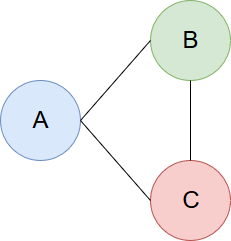
\includegraphics[width=0.5\textwidth]{pictures/ejemplo.png}
        \caption{Grafo de ejemplo con una solución válida}
    \end{figure}
	
    \begin{figure}[H]
        \centering
        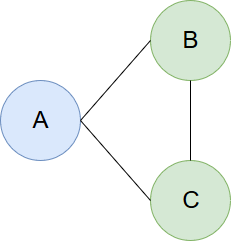
\includegraphics[width=0.5\textwidth]{pictures/ejemplobad.png}
        \caption{Grafo de ejemplo con una solución inválida}
    \end{figure}

	Concretamente, hemos empleado el grafo de Petersen. Hemos variado ligeramente 
    la numeración de los nodos. Para mayor comodidad, el primer nodo lo hemos numerado como '1' en lugar de '0' y así sucesivamente (es decir, 
    hemos incrementado en 1 el valor de cada nodo.)

    \begin{figure}[H]
        \centering
        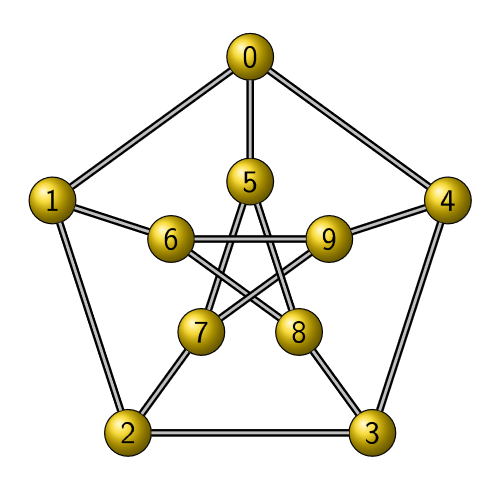
\includegraphics[width=0.5\textwidth]{pictures/PetersenGraph.png}
        \caption{Grafo de Petersen}
    \end{figure}

    Para encontrar la solución de este problema se ha empleado el problema 3-SAT. 
    El problema SAT fue uno de los primers en descubrirse NP-completo. Dicho problema consiste 
    en dada una ecuación booleana, encontrar los valores para los cuales es verdadera. Además, la 
    ecuación debe tener las siguientes características: 
    \begin{itemize}
        \item La ecuación global se compone de ecuaciones enlazadas con la puerta logica and
        \item Cada subecuación esta compuesta por variables ($x_1, x_2, ...$) unidas por la puerta lógica OR.
    \end{itemize}

    A continuación podemos ver una ecuación para el problema SAT:
        \[ ( x_1 \vee x_2 \vee x_3) \wedge (x_3 \vee x_4)\]

    
\section{Methodology}
    La implementación de la práctica se ha realizado en C++, hemos dividido el programa en varias partes. 
    \subsubsection{Lectura del grafo}
        Para la lectura del grafo nos hemos apoyado en un fichero. Dicho fichero debe tener la siguiente estructura:
        \begin{itemize}
            \item La definición de cada nodo se realiza en una fila. 
            \item Los nodos a los que esta conectado el nodo que estamos definiendo estan separados por comas. 
        \end{itemize}
        
        De esta manera realizamos la lectura del grafo, representado mediante listas de adyacencia.
        A continuación podemos ver el fichero con el grafo de ejemplo de la sección anterior.
        %Insertar fichero con el grafo de ejemplo.
        \begin{figure}[H]
            \centering
            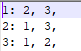
\includegraphics[width=0.2\textwidth]{pictures/entrada_ejemplo.png}
            \caption{Fichero de entrada para el grafo de ejemplo}
        \end{figure}

        De igual manera, el grafo de Petersen representado mediante listas de adyacencia. 
        \begin{figure}[H]
            \centering
            \includegraphics[width=0.2\textwidth]{pictures/petersen_modificado.png}
            \caption{Fichero de entrada para el grafo de Petersen}
        \end{figure}
    
    \subsubsection{Transformación del 3-Col to SAT}
        Lo primero al realizar esta parte ha sido analizar profundamente la estructura de las ecuaciones booleanas que 
        representan al grafo que deseamos colorear.
        Estas ecuaciones se pueden dividir en dos grupos.
        \begin{itemize}
            \item Ecuaciones correspondientes al color del propio nodo.
            \item Ecuaciones correspondientes al color de los nodos adyacentes al nodo actual.
        \end{itemize}
        %Remarcar que por eficiencia temporal las aristas se escriben dobles, cosa que no afecta a picosat.
        Si nos fijamos, en los grafos que hemos empleado las aristas son bidireccionales. Bastaría con definirlas una sola vez, 
        sin embargo, para mantener la legibilidad del código he decicido permitir que se escriban dos veces (una en cada sentido).
        Este aumento en número de ecuaciones no afecta a PicoSAT. A continuación mostramos la salida para el grafo de Petersen 
        %Insertar imagen grafo Petersen.
    
    \subsubsection{Escritura de las ecuaciones booleanas}
        Finalmente es necesario escribir en un fichero las ecuaciones correspondientes al grafo. Estas 
        ecuaciones deben ir en formato DIMACS. El fin de este formato es el correcto procesamiento por parte del 
        programa PicoSAT. 

        Simplemente en lugar de ir mostrando las ecuaciones por la salida estándar las hemos dirigido hacia una cadena. Igualmente 
        hemos definido una variable que se encarga de contar cuantas ecuaciones tiene y otra más para el número de variables. 
        Volcando las cadenas y los contadores en un fichero conseguimos tener la información lista para PicoSAT.

        El programa ha sido paramétrizado de tal forma que tanto el grafo como el número de colores pueda modificarse.  
    
    \subsubsection{PicoSAT}
        Finalmente, para ejecutar el programa hemos empleado la orden: \\
         \vspace{5mm} $./picosat$ salida \\

        Si deseamos ver todas las soluciones \\
         \vspace{5mm} $./picosat$ --all salida


\section{Results and Discussion}
    Para averiguar el tipo de reducción obtenida hemos realizado un estudio de la complejidad temporal del programa 3SAT (es decir, 
    suponiendo que el numero de colores es 3). 
    \begin{figure}[H]
        \centering
        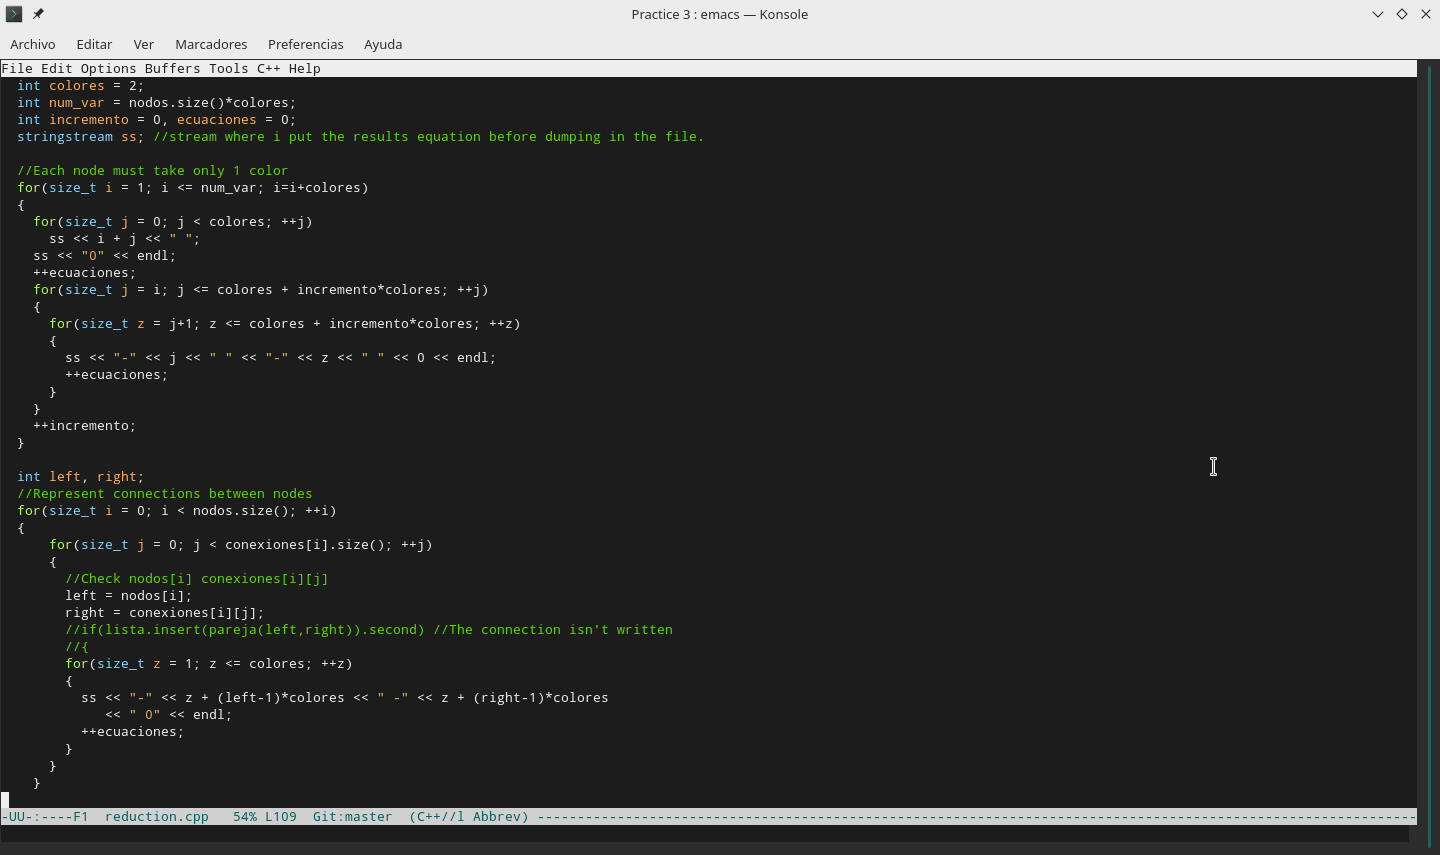
\includegraphics[width=1\textwidth]{pictures/analisis.png}
        \caption{Análisis temporal del algoritmo}
    \end{figure}
    Como se puede observar, existen dos anidamientos de bucles for. Por tanto, hemos decidido dividir en análisis en dos bloques, 
    cada uno correspondiente a un bloque de bucles for. 

    Analizando el comportamiento de los bucles, vemos que el número de iteraciones depende de dos factores: 
    \begin{itemize}
        \item Número de nodos: n.
        \item Número de colores: en este caso es 3.
    \end{itemize}
    En primer anidamiento distinguimos 4 bucles for:
    \begin{itemize}
        \item for(size\_t i = 1; i $\leq$ num\_var; i = i + colores): Este bucle se ejecuta n veces
        \item for(size\_t j = 0; j $<$ colores; ++colores): Este bucle se ejecuta colores veces
        \item for(size\_t j = 0; j $\leq$ colores + incremento*colores; ++j): Este bucle se ejecuta colores veces
        \item for(size\_t z = j+1; z $\leq$ colores + incremento*colores; ++z): Este bucle se ejecuta j-1 veces
    \end{itemize}
    
    Por tanto, la complejidad de la primera parte es 
    \[t(n) = n(3+3*1) = n\]
    Pasamos a analizar la segunda parte del algoritmo. Distinguimos los siguientes bucles
    \begin{itemize}
        \item for(size\_t i = 0; i < nodos.size(); ++i): Se ejecuta n veces
        \item for(size\_t j = 0; j < conexiones[i].size(); ++j): Se ejecuta tantas veces como aristas tenga el grafo. En el caso peor (n-1) veces.
        \item for(size\_t z = 1; z <= colores; ++z): Se ejecuta 3 veces.
    \end{itemize}
    
    Por tanto, la complejidad de la segunda parte es:
    \[t(n) = n((n-1)*3) = n^2\]
    
    Fusionando ambas partes, por la regla del máximo tenemos que el algoritmo tiene un orden $O(n) = n^2$, es decir, posee un orden polinómico. Nuestro programa posee una complejidad polinómica. Consecuentemente hemos obtenido una reducción polinómica.
    Empleando tres colores, obtenemos las ecuaciones: 
    %Insertar fichero de ecuaciones. 
    
    Una solución para el grafo de Petersen es esta: 
    \begin{figure}[H]
            \centering
            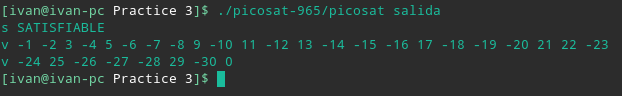
\includegraphics[width=0.5\textwidth]{pictures/solution.png}
            \caption{Fichero de entrada para el grafo de Petersen}
        \end{figure}
        
    Así mismo, todas las posibles soluciones son: 
    %Insertar la solución de las ecuaciones booleanas, no te compliques coloreando el grafo.
    \begin{figure}[H]
            \centering
            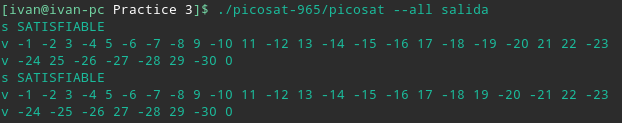
\includegraphics[width=0.5\textwidth]{pictures/solution_all.png}
            \caption{Fichero de entrada para el grafo de Petersen}
    \end{figure}
        
    En cambio, no existe ninguna solución si decrementamos el numero de colores a 2.
    Finalmente, analizando la estructura del grafo tenemos que el Clique Máximo del grafo de Petersen es de tamaño 2.  

    El Clique máximo del grafo es 2. Así mismo no podemos colorear el grafo con menos de tres colores. Esto, intuitivamente nos sugiere que 
    \[clique < numero_colores\]

Siendo clique el numero de nodos que forman el máximo clique y numero\_colores el número 
de colores mínimo necesario para colorear el grafo. Ahora a 
fin de contrastar esta suposición, decidimos probar con el grafo de ejemplo que hemos mostrado al principio del report. 
%Insertar imagen 
\begin{figure}[H]
    \centering
    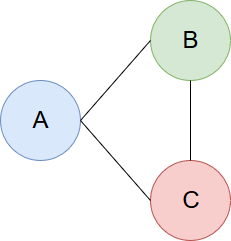
\includegraphics[width=0.5\textwidth]{pictures/ejemplo.png}
    \caption{Grafo de ejemplo}
\end{figure}

Aquí, sin embargo, el clique máximo del grafo es 3 y se puede colorear correctamente con tres colores. Por tanto tenemos que:
    \[clique \leq numero_colores\]
    
Consecuentemente, realizamos un intento de colorear el grafo de Petersen con dos colores 
\begin{figure}[H]
    \centering
    \includegraphics[width=0.5\textwidth]{pictures/interior.png}
    \caption{Interior del grafo de Petersen}
\end{figure}

No ha hecho falta colorear todo el grafo, trabajando únicamente con el interior podemos observar que no es coloreable con sólo dos colores, el nodo
numero 9 no puede tomar ni rojo ni verde.   
Por tanto la estructura del grafo también influye en el número mínimo de colores necesarios. Si quereremos ceñirnos estrictamente al Clique 
para estimar el número de colores, tenemos que 
    \[clique < numero_colores \] 

Aunque en algunos casos es posible que se cumpla: 
    \[clique \leq numero_colores\]

\section{Conclussion}

    
\bibliography{bibliografia} 
\bibliographystyle{unsrt}

\end{document}
